\begin{figure}[t]
\centering
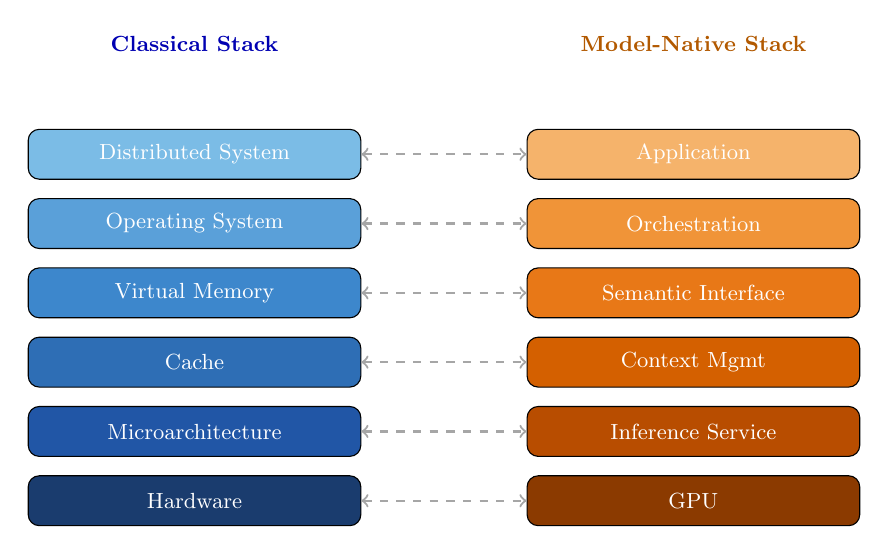
\begin{tikzpicture}[
    scale=0.88, transform shape,
    cbox/.style={
        draw, rounded corners=4pt, minimum width=4.8cm, minimum height=0.72cm,
        font=\small, text=white, align=center, inner sep=3pt
    },
    mbox/.style={
        draw, rounded corners=4pt, minimum width=4.8cm, minimum height=0.72cm,
        font=\small, text=white, align=center, inner sep=3pt
    },
    arr/.style={<->, dashed, thick, gray!70},
    clabel/.style={font=\small\bfseries, text=blue!70!black},
    mlabel/.style={font=\small\bfseries, text=orange!70!black}
]

% Classical stack colors (blue shades, bottom to top: dark to light)
\definecolor{c1}{HTML}{1A3C6E}
\definecolor{c2}{HTML}{2156A6}
\definecolor{c3}{HTML}{2E6EB5}
\definecolor{c4}{HTML}{3D87CC}
\definecolor{c5}{HTML}{5AA0D9}
\definecolor{c6}{HTML}{7BBCE6}

% Model-native stack colors (orange shades, bottom to top: dark to light)
\definecolor{m1}{HTML}{8B3A00}
\definecolor{m2}{HTML}{B84D00}
\definecolor{m3}{HTML}{D46000}
\definecolor{m4}{HTML}{E87817}
\definecolor{m5}{HTML}{F09438}
\definecolor{m6}{HTML}{F5B36B}

% Column labels
\node[clabel] at (-3.6, 6.6) {Classical Stack};
\node[mlabel] at ( 3.6, 6.6) {Model-Native Stack};

% Classical stack (left column, bottom = layer 1)
\node[cbox, fill=c1] (cl1) at (-3.6, 0.0) {Hardware};
\node[cbox, fill=c2] (cl2) at (-3.6, 1.0) {Microarchitecture};
\node[cbox, fill=c3] (cl3) at (-3.6, 2.0) {Cache};
\node[cbox, fill=c4] (cl4) at (-3.6, 3.0) {Virtual Memory};
\node[cbox, fill=c5] (cl5) at (-3.6, 4.0) {Operating System};
\node[cbox, fill=c6] (cl6) at (-3.6, 5.0) {Distributed System};

% Model-native stack (right column, bottom = layer 1)
\node[mbox, fill=m1] (ml1) at ( 3.6, 0.0) {GPU};
\node[mbox, fill=m2] (ml2) at ( 3.6, 1.0) {Inference Service};
\node[mbox, fill=m3] (ml3) at ( 3.6, 2.0) {Context Mgmt};
\node[mbox, fill=m4] (ml4) at ( 3.6, 3.0) {Semantic Interface};
\node[mbox, fill=m5] (ml5) at ( 3.6, 4.0) {Orchestration};
\node[mbox, fill=m6] (ml6) at ( 3.6, 5.0) {Application};

% Horizontal dashed arrows between corresponding layers
\draw[arr] (cl1.east) -- (ml1.west);
\draw[arr] (cl2.east) -- (ml2.west);
\draw[arr] (cl3.east) -- (ml3.west);
\draw[arr] (cl4.east) -- (ml4.west);
\draw[arr] (cl5.east) -- (ml5.west);
\draw[arr] (cl6.east) -- (ml6.west);

\end{tikzpicture}
\caption{Layer comparison: classical computing stack vs model-native computing stack}
\label{fig_dual_stack}
\end{figure}
